\documentclass[pdflatex,iicol,sn-basic,Numbered]{sn-jnl}
\usepackage[T1]{fontenc}
\usepackage{lmodern,amsmath,amssymb,booktabs,graphicx,xurl,microtype}
\IfFileExists{spanish.ldf}{\usepackage[spanish,es-tabla,es-nodecimaldot]{babel}}{\usepackage[provide=*,spanish]{babel}}
\AtBeginDocument{\renewcommand{\tablename}{Tabla}\renewcommand{\figurename}{Figura}}
\raggedbottom
\begin{document}
\hypersetup{pdftitle={Sonificación de estados cuánticos mediante geometría de Bloch y grafos de información mutua},pdfauthor={}}
\title{Sonificación de estados cuánticos mediante geometría de Bloch y grafos de información mutua}
% Insertar nombres y afiliaciones verificados antes del envío.
\abstract{Sonificar un estado multiqubit exige elegir qué descriptores cuánticos organizarán el sonido y establecer qué información sobrevive a esa elección. Presentamos un motor determinista que combina geometría local de Bloch con un bosque de expansión máxima de información mutua por pares. Los descriptores de cada qubit controlan voces sinusoidales; los modos de recorrido en anchura y profundidad las organizan en fronteras simultáneas o eventos secuenciales. Evaluamos 100 circuitos de desarrollo y 100 circuitos reservados prospectivamente, de 15 qubits y profundidades 0--10, con 2.200 instantáneas de estado y 4.400 salidas primarias. Los análisis consideran profundidad y observaciones repetidas. En validación, añadir resúmenes de información mutua reduce un 82,01\% el error cuadrático medio de predicción de duración del modo en profundidad, con error de raíz cuadrática media de 46,65 a 19,78 milisegundos. Los controles sintéticos del bosque explican este resultado: dicha duración permanece invariante al cambiar conexiones y ubicación de pesos conservando sus multiconjuntos por componente; la duración en anchura cambia. Se replican asociaciones débiles entre distancias de Bloch y audio, pero no la asociación exploratoria de información mutua. Una familia física continua tiene reducciones de uno y dos qubits y audio final idénticos por modo, mientras la entropía del corte central recorre 0--7 bits. Los resultados caracterizan sensibilidad a descriptores seleccionados y un límite preciso de inferencia global. El instrumento proporciona un componente auditivo trazable para exploración audiovisual y composición; sus beneficios perceptuales, de usabilidad y educativos no se han evaluado.}
\keywords{Sonificación cuántica, Geometría de Bloch, Información mutua, Representación auditiva, Interfaces multimodales, Reproducibilidad}
\maketitle

\section{Introducción}\label{sec:introduction}
La computación cuántica suele representarse mediante circuitos, amplitudes y distribuciones de probabilidad. Convertir aspectos seleccionados de esta estructura en sonido plantea un problema de representación: ¿qué relaciones matemáticas se convierten en relaciones acústicas y qué información se pierde? La sonificación por mapeo de parámetros conecta variables de los datos con controles de síntesis como frecuencia, amplitud y posición espacial \citep{GrondBerger2011}. En un estado multiqubit, esta elección es decisiva. Su descripción completa crece exponencialmente con el número de qubits, mientras un conjunto compacto de descriptores locales y por pares puede inspeccionarse y recibir funciones acústicas explícitas.

Estas funciones también definen una forma sonora. Simultaneidad, sucesión, envolventes y organización espacial determinan cómo se combinan las contribuciones; por ello, el diseño sonoro forma parte de la representación. Vickers y Hogg sitúan las intenciones informativas y artísticas en un espacio compartido de práctica de sonificación \citep{VickersHogg2006}. Aquí, la motivación compositiva se refiere a restricciones explícitas, condicionadas por los datos, sobre las voces y su organización temporal. Sus consecuencias computacionales pueden medirse sin considerar demostradas la calidad estética o la comprensión del oyente.

La integración de sonificación y visualización ofrece un contexto para hacer inspeccionables estas correspondencias \citep{Enge2024}. Una bola de Bloch y un grafo de correlaciones pueden mostrar los descriptores que también controlan el sonido. SingingFunction ilustra otra representación auditiva de estructura matemática con exploración interactiva y evaluación con oyentes \citep{GrondHermann2012}. Nuestro aporte presente se refiere al motor auditivo y su caracterización computacional. Establece qué puede explicar legítimamente una interfaz visual futura o complementaria, sin aportar evidencia de reconocimiento humano, usabilidad o aprendizaje.

La sonificación cuántica ya comprende distintos objetivos de representación. Kontogeorgakopoulos y Burgarth sonifican dinámica cuántica controlada simulada mediante mapeo de parámetros y composición electroacústica \citep{Kontogeorgakopoulos2014}. Q1Synth conecta un instrumento interactivo de esfera de Bloch con vectores de estado y resultados de medición de qubits \citep{Miranda2023}. El Variational Quantum Harmonizer relaciona optimización variacional y organización musical; el capítulo previo a publicación consultado describe este marco.\footnote{P.~V. Itabora\'i et al., ``Developing a Framework for Sonifying Variational Quantum Algorithms: Implications for Music Composition'', capítulo previo a publicación, arXiv:2409.07104 (2024), \url{https://arxiv.org/abs/2409.07104}.} El preprint de Christie y Trayford mapea, en cambio, estructura de matrices de densidad y coherencia en dinámica de sistemas abiertos.\footnote{R. Christie y J. Trayford, ``The Sound of Decoherence'', arXiv:2412.17045 (2024), \url{https://arxiv.org/abs/2412.17045}.} Tudoce y colaboradores combinan representaciones colectivas de Husimi y entropía de entrelazamiento bipartito en dinámica multiqubit \citep{Tudoce2026}. Estos antecedentes impiden afirmar una primera sonificación cuántica o multiqubit. Sus objetivos también difieren lo suficiente como para que comparar arquitecturas no establezca una clasificación de rendimiento.

Nuestro motor separa control local de las voces y secuenciación relacional. Las reducciones de un qubit proporcionan radio y dirección de Bloch; la información mutua cuántica por pares proporciona un grafo ponderado de correlaciones totales, incluidas contribuciones clásicas y cuánticas \citep{Groisman2005}. Un bosque de expansión máxima selecciona parte de estas relaciones para organizar eventos. El recorrido en anchura (BFS) agrupa qubits en fronteras simultáneas; el recorrido en profundidad (DFS) los reproduce secuencialmente. Los modos también difieren en promedio de voces, duraciones de evento y ataques de envolvente. Su comparación se refiere, por tanto, a configuraciones completas de síntesis. ``Topología'' designa aquí conectividad de un grafo etiquetado, sin aludir a una fase topológica de la materia ni a geometría del espacio-tiempo.

Una ecuación de mapeo no establece por sí sola una asociación en los descriptores acústicos finales. El solapamiento de osciladores y la secuenciación pueden alterar características agregadas. La profundidad del circuito puede afectar tanto a descriptores cuánticos como al sonido, produciendo correlaciones agrupadas ausentes dentro de cada profundidad. Además, una buena predicción desde descriptores hacia audio es compatible con una representación irreversible. Nuestra pregunta central es operacional: \emph{¿qué descriptores locales y relacionales seleccionados tienen consecuencias acústicas medibles en este conjunto de circuitos y qué no puede identificar la representación?}

Cinco preguntas de investigación conservan la organización estadística del proyecto, con definiciones corregidas para las observaciones repetidas:
\begin{enumerate}
\item[\textbf{RQ1.}] Tras retirar las medias específicas de cada profundidad, ¿se asocian radio medio de Bloch y ángulo polar ponderado por radio con RMS y centroide espectral, respectivamente, en cada modo?
\item[\textbf{RQ2.}] ¿Cómo varían geometría local, entropías de subsistemas, correlaciones por pares y descriptores acústicos con la profundidad?
\item[\textbf{RQ3.}] En cada profundidad no inicial y modo, ¿se asocia la varianza circular azimutal ponderada por radio con la correlación de canales estéreo?
\item[\textbf{RQ4.}] ¿Cómo difieren las dos configuraciones completas para el mismo estado en duración, RMS, centroide, ancho de banda, entropía espectral y flujo espectral?
\item[\textbf{RQ5.}] ¿Añadir resúmenes de información mutua mejora la predicción de audio desde descriptores, respecto de profundidad y resúmenes locales, en semillas de circuito nuevas?
\end{enumerate}

Respondemos mediante una cohorte de desarrollo y otra de validación independiente, especificada prospectivamente. Los análisis complementarios de distancias y controles sintéticos del bosque caracterizan sensibilidad y mecanismo. Finalmente, un argumento constructivo de identificabilidad proporciona estados físicos con distinto entrelazamiento central y audio idéntico. El aporte es esta combinación de instrumento explícito, comportamiento acústico evaluado de manera independiente y límite demostrable de representación; no un teorema general de que el sonido conserve información cuántica.

\section{Metodología}\label{sec:methods}
\subsection{Circuitos y unidades experimentales}
El estudio principal utiliza 100 semillas de desarrollo (1000--1099) y 100 de validación (3000--3099). Cada semilla genera una trayectoria ideal de 15 qubits desde $|0\rangle^{\otimes15}$, con instantáneas a profundidades $d=0,\ldots,10$. Cada capa no inicial aplica compuertas de un qubit seleccionadas aleatoriamente entre $\sqrt X$, $\sqrt Y$ y $\sqrt W$, excluyendo repeticiones consecutivas por qubit, seguidas de $\operatorname{fSim}(\pi/2,\pi/6)$ entre vecinos de una cadena unidimensional. Alternan los emparejamientos $(0,1),(2,3),\ldots$ y $(1,2),(3,4),\ldots$. Un generador privado con semilla garantiza consistencia de prefijos. Se trata de un conjunto unidimensional especificado, no de reconstruir un procesador bidimensional ni de un experimento de ventaja cuántica.

La simulación clásica exacta por vector de estado produce estados globalmente puros, sin mediciones, shots ni ruido. La mezcla local aparece por traza parcial y no prueba decoherencia ambiental. Cada cohorte contiene 1.100 instantáneas y 2.200 salidas primarias BFS/DFS. El total principal es de 200 semillas independientes, 2.200 instantáneas y 4.400 salidas; capas y modos son observaciones repetidas. Una cohorte examinada previamente (2000--2099) y otras extensiones exploratorias anteriores no se utilizaron como conjunto prospectivo de prueba ni se agregaron a estos totales. También se excluye el piloto técnico de semillas 0--2.

La especificación de validación quedó congelada en el commit \texttt{e968ba6} antes de generar 3000--3099. Es una congelación local auditable, no un prerregistro público. El sintetizador corresponde al commit de referencia \texttt{bb31388}, etiqueta \texttt{paper-pipeline-v1.0.0}; el protocolo y hashes completos se incluyen en el Recurso en línea 2. No se modificó ninguna regla de síntesis para la validación. Las 100 ejecuciones pasaron la validación técnica registrada del pipeline; ninguna semilla fallida fue sustituida ni excluida de la cohorte analizada.

\subsection{Descriptores cuánticos}
La reducción del qubit $i$ es
\begin{equation}
\rho_i=\tfrac12(\mathbb I+\mathbf b_i\cdot\boldsymbol\sigma),\qquad r_i=\|\mathbf b_i\|\in[0,1].
\end{equation}
Su dirección es $(\theta_i,\phi_i)$ cuando está definida. La pureza y la entropía lineal normalizada satisfacen
\begin{equation}
\operatorname{Tr}\rho_i^2=(1+r_i^2)/2,\qquad L_i=1-r_i^2.
\end{equation}
Son descriptores matemáticamente dependientes, no recursos cuánticos independientes. Los resúmenes direccionales ponderados usan $w_i=r_i\mathbf1\{r_i>10^{-10}\}$:
\begin{align}
\bar\theta_r&=\frac{\sum_i w_i\theta_i}{\sum_i w_i},\\
V_\phi&=1-\left|\frac{\sum_i w_i e^{\mathrm i\phi_i}}{\sum_i w_i}\right|.
\end{align}
Ambos se definen como cero si el denominador se anula. Las entropías locales de von Neumann se expresan en bits.

La información mutua cuántica por pares es
\begin{equation}
I_{ij}=S(\rho_i)+S(\rho_j)-S(\rho_{ij}),\quad 0\le I_{ij}\le2.
\end{equation}
Se calculan los 105 pares y se retienen aristas con $I_{ij}>10^{-10}$ bits. Los residuos numéricos negativos dentro de la tolerancia se recortan; valores inferiores a $-10^{-8}$ producen error. La matriz completa se guarda separadamente del bosque de expansión máxima. Los resúmenes incluyen total retenido $I_{\rm tot}$ y entropía de pesos
\begin{equation}
H_E=-\sum_{e:p_e>0}p_e\log_2p_e,\qquad p_e=I_e/I_{\rm tot},
\end{equation}
con $H_E=0$ si el grafo está vacío. $H_E$ describe distribución de pesos; no es entropía de entrelazamiento bipartito.

La bipartición central es $A=\{0,\ldots,6\}$ y $B=\{7,\ldots,14\}$. Como el estado global es puro, $S_A=S(\rho_A)$ mide entrelazamiento en ese corte, con $0\le S_A\le7$ bits. Se calcula para análisis pero no entra directamente a la síntesis. No debe confundirse $S_A$ ni información mutua con entropía espectral.

\subsection{Mapeo y secuenciación congelados}\label{sec:mapping}
La Fig.~\ref{fig:architecture} separa las vías de descriptores. Cada qubit controla una voz sinusoidal con
\begin{align}
f_i&=110\,8^{\theta_i/\pi}\ \mathrm{Hz},\\
a_i&=0.22(0.12+0.88r_i),\qquad m_i=0.30L_i.
\end{align}
Antes de envolvente y ganancias estéreo, la señal es
\begin{equation}
s_i(t)=a_i[1+m_i\sin(2\pi\,6t)]\sin(2\pi f_it).
\end{equation}
El azimut fija ganancias de potencia igual mediante $p_i=(\phi_i\bmod2\pi)/(2\pi)$, $g_{Li}=\cos(\pi p_i/2)$ y $g_{Ri}=\sin(\pi p_i/2)$. Cambia ganancias espaciales, no fase portadora. Para $r_i\le10^{-8}$ el sintetizador sustituye $\theta_i=\pi/2$, $\phi_i=\pi$: una dirección neutra audible cuando el ángulo físico es indefinido. Este umbral difiere del $10^{-10}$ usado en resúmenes direccionales.

\begin{figure*}[t]
\centering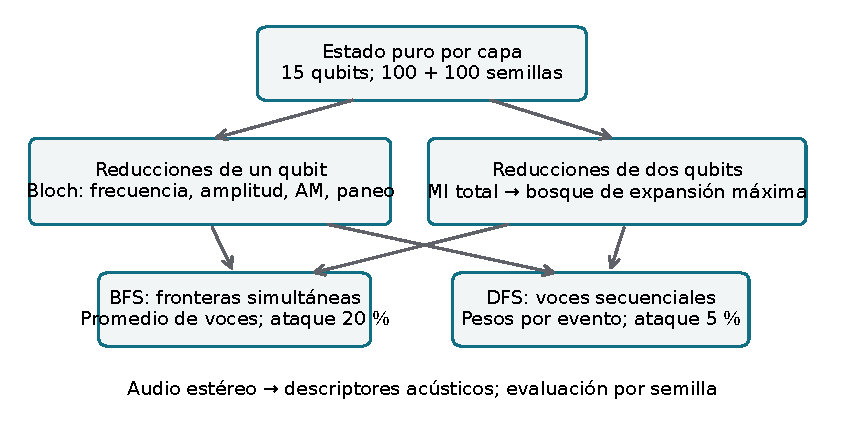
\includegraphics[width=\textwidth]{figures/Fig1_es.pdf}
\caption{Vías de descriptores del motor congelado. Las reducciones locales controlan voces y el grafo de información mutua selecciona el bosque para secuenciarlas. Ambas vías reciben la misma instantánea. Es un esquema algorítmico, no una captura de la interfaz audiovisual}\label{fig:architecture}
\end{figure*}

La raíz preferida de cada componente es el qubit 7 si está presente y, en otro caso, la etiqueta mínima. Primero se visita la componente de la raíz preferida y luego las restantes por etiqueta mínima. Los vecinos se ordenan por peso decreciente y después por etiqueta. Estas elecciones fijan un recorrido determinista dependiente de etiquetas; no se supone invariancia frente a reetiquetar qubits.

Una raíz dura 0,30 s; una arista entrante de peso $w$ fija $\tau(w)=0.60-0.25w$ s usando el intervalo físico constante $[0,2]$ bits. Hay 0,12 s de silencio entre componentes. DFS reproduce cada voz por separado, con su peso entrante y una envolvente lineal de ataque/decaimiento cuyo ataque ocupa el 5\%. BFS reproduce simultáneamente las voces de una frontera, dividiendo su suma por el tamaño de la frontera, usando el promedio de pesos entrantes positivos para su duración y un ataque del 20\%. Cada evento se redondea individualmente a muestras a 22.050 Hz. No hay normalización de pico ni RMS por archivo; el promedio de frontera pertenece a BFS. Los WAV de coma flotante conservan amplitud digital. Las mezclas combinadas y archivos continuos son auxiliares de escucha y se excluyen de la estadística primaria.

\subsection{Extracción acústica}
La transformada de Fourier de tiempo corto (STFT) utiliza ventana Hann de 2.048 muestras y solapamiento de 1.536, sin extensión de bordes ni relleno final. La potencia por cuadro es $P_{kt}=(|X_{L,kt}|^2+|X_{R,kt}|^2)/2$. Centroide y ancho de banda son media y desviación estándar de frecuencia ponderadas por potencia. La entropía espectral es $-\sum_k u_{kt}\log_2(u_{kt}+10^{-15})$, donde $u_{kt}=P_{kt}/\sum_kP_{kt}$; los cuadros sin potencia toman valor cero. El flujo es distancia euclidiana entre espectros consecutivos de potencia normalizada. Cada descriptor espectral se promedia entre cuadros sin retirar silencios ni ponderarlos por energía.

La duración es número de muestras entre frecuencia de muestreo. El RMS conjunto es $\sqrt{\langle(L^2+R^2)/2\rangle}$; la correlación estéreo es Pearson entre canales y toma cero si alguno tiene varianza nula. El balance es $(\mathrm{RMS}_R-\mathrm{RMS}_L)/(\mathrm{RMS}_R+\mathrm{RMS}_L+10^{-15})$. Son descriptores digitales, no estimaciones de presión sonora calibrada, energía acústica en julios, sonoridad percibida ni discriminación humana.

\subsection{Especificación estadística}
Los resultados de desarrollo informaron las preguntas corregidas y el objetivo primario. Los modelos, variables, capas y tamaño de validación posterior quedaron congelados. La unidad independiente de remuestreo es la trayectoria completa de una semilla. Las familias separadas de pruebas usan ajuste Benjamini--Hochberg (BH) de tasa de descubrimientos falsos \citep{Benjamini1995}; $q$ designa valores corregidos. No constituyen una única familia controlada globalmente para todo el artículo.

RQ1 centra cada variable dentro de su profundidad y calcula Pearson sobre los residuos agrupados, por modo. Resume covarianza dentro de profundidades; no afirma significación individual en todas ellas. Las 5.000 permutaciones de etiquetas de semilla conservan trayectorias; un bootstrap de 5.000 remuestreos de semillas recalcula el centrado para intervalos de confianza (IC). BH incluye cuatro asociaciones. RQ2 presenta medias por profundidad e IC del 95\% puntuales por bootstrap, no bandas simultáneas.

RQ3 calcula Spearman entre 100 semillas en cada profundidad 1--10 y modo. Se excluye la capa 0 por degeneración. Cada una de las 20 pruebas utiliza 100.000 permutaciones de etiquetas y BH sobre las 20. RQ4 promedia las 11 diferencias pareadas BFS menos DFS dentro de cada semilla, antes de una prueba $t$ pareada con 99 grados de libertad. Presenta IC con 10.000 remuestreos y BH sobre seis descriptores. Las tablas completas por capa y de controles figuran en el Recurso en línea 1.

RQ5 ajusta mínimos cuadrados ordinarios por modo y objetivo, con duración y flujo espectral como objetivos. $M_0$ contiene intercepto y profundidad categórica; $M_1$ añade $\bar r$, $\bar L$, $\bar\theta_r$ y $V_\phi$; $M_2$ añade $\log(1+I_{\rm tot})$ y $H_E$. Escalado y coeficientes se ajustan sólo en desarrollo. Los modelos quedan fijos para una única evaluación en validación: se predice audio desde descriptores cuánticos, no se decodifica el estado desde audio.

El único resultado primario es la mejora de duración DFS,
\begin{equation}
\Delta=\mathrm{MSE}(M_1)-\mathrm{MSE}(M_2).
\end{equation}
En cada semilla de prueba se promedian errores cuadrados sobre las 11 profundidades; 5.000 remuestreos de esos 100 promedios dan un IC del 95\%. El criterio congelado es límite inferior positivo. El IC está condicionado al entrenamiento y ajuste fijos, no a repetir todo el entrenamiento. La reducción relativa es $100\Delta/\mathrm{MSE}(M_1)$. Las otras tres combinaciones modo/objetivo son secundarias, con IC puntuales y sin interpretación confirmatoria conjunta. El Recurso en línea 2 registra semillas de generadores y ajustes.

\subsection{Asociaciones de distancias y controles del bosque}
El análisis complementario de distancias utiliza ocho variables acústicas: los seis descriptores de RQ4 más balance y correlación estéreo, estandarizados por modo con medias y desviaciones estándar poblacionales de desarrollo. Dentro de cada profundidad elegible, compara distancias euclidianas acústicas con (i) promedio de 15 distancias cartesianas de Bloch alineadas por qubit y (ii) distancia euclidiana entre las 105 entradas del triángulo superior de información mutua. El estadístico es promedio no ponderado de correlaciones Spearman entre distancias por profundidad. La misma permutación de semillas se aplica en todas las profundidades de cada una de 5.000 permutaciones. Los 4.950 pares son dependientes; el tamaño muestral sigue siendo 100 semillas. BH cubre cuatro pruebas y Benjamini--Yekutieli (BY) evalúa sensibilidad a dependencia \citep{Benjamini2001}. Se excluyen distancias con rango numérico inferior a $10^{-10}$: Bloch usa profundidades 1--10 e información mutua 2--10. No se presenta IC por bootstrap de distancias ni afirmación de isometría. Como la duración es una variable acústica, estas pruebas no aíslan geometría espectral de organización temporal.

Los controles conservan entradas de Bloch, conjuntos de nodos por componente y multiconjuntos de pesos. \emph{Permutar pesos} los redistribuye sobre las mismas aristas. \emph{Permutar árbol} muestrea un árbol etiquetado mediante una secuencia de Pr\"ufer uniforme por componente y permuta pesos sobre sus aristas, cambiando conectividad y ubicación conjuntamente. No conserva grados ni distancias del grafo. Se seleccionan profundidades 2, 3, 6 y 10; las 100 semillas reciben 20 réplicas de cada control en ambos modos. Incluyendo originales, son 32.800 síntesis y 32.000 comparaciones. Se promedian réplicas por estado y profundidades seleccionadas por semilla, antes de 5.000 remuestreos de semillas. Las observaciones previstas son duración y fronteras BFS e invariancia de duración DFS; los demás descriptores son exploratorios y se reportan juntos con IC puntuales. Estos bosques sintéticos prueban el sintetizador, no matrices de información mutua nuevas físicamente realizables ni nuevas simulaciones cuánticas.

\subsection{Integridad de implementación y diagnósticos analíticos}
La auditoría verifica cuadrículas completas, semillas disjuntas, consistencia cuántica entre modos, valores finitos, hashes, reconstrucción de predicciones y concordancia de estadística registrada e independiente. Coinciden los 1.334 hashes del paquete de cierre; sus cinco archivos \texttt{src} son idénticos byte a byte a la referencia archivada. La reconstrucción del audio de desarrollo desde descriptores guardados había pasado antes de la validación. Para la cohorte nueva, vectores de estado y WAV originales no forman parte del paquete compacto: el pipeline registra su validación por ejecución y la auditoría independiente de cierre verifica matrices, descriptores, tablas y código suministrados. El entorno efectivo de validación registra Python 3.11.14, NumPy 2.3.5, SciPy 1.17.1, NetworkX 3.6.1 y Qiskit 2.3.0.

Dos diagnósticos analíticos complementan las estadísticas: identidades exactas de duración derivadas de la secuenciación y una familia física externa que demuestra no identificabilidad de entropía del corte desde audio de la instantánea final. No son circuitos adicionales del conjunto RQC. Un cálculo de discontinuidad de coordenadas evalúa continuidad del paneo congelado. Las derivaciones y certificados completos aparecen en el Recurso en línea 1.

\section{Resultados}\label{sec:results}
\subsection{Asociaciones locales y trayectorias por profundidad}
Las cuatro asociaciones de RQ1 se replican (Tabla~\ref{tab:rq1}). Radio--RMS es mucho más fuerte en DFS que BFS, coherente con voces separadas frente a solapadas y promediadas; la tabla no constituye una comparación causal aislada de algoritmos de recorrido. El ángulo polar ponderado se asocia fuertemente con centroide en ambos modos, sin ser una fórmula del centroide.
\begin{table*}[t]
\caption{RQ1 en validación: Pearson tras centrar por profundidad. IC del 95\% por semilla y BH en cuatro pruebas; 5.000 permutaciones limitan la resolución del valor de prueba.}\label{tab:rq1}
\centering\small
\begin{tabular}{llrrr}
\toprule
Modo & Relación & $r$ & IC del 95\% & $q$ \\
\midrule
BFS & $\bar r$--RMS & $0.449$ & $[0.389, 0.500]$ & $0.000200$ \\
BFS & $\bar\theta_r$--centroide & $0.745$ & $[0.710, 0.777]$ & $0.000200$ \\
DFS & $\bar r$--RMS & $0.979$ & $[0.972, 0.985]$ & $0.000200$ \\
DFS & $\bar\theta_r$--centroide & $0.753$ & $[0.717, 0.784]$ & $0.000200$ \\
\bottomrule
\end{tabular}
\end{table*}


La Fig.~\ref{fig:depth} presenta tres trayectorias descriptivas. La entropía media del corte asciende en pasos alternos hasta 6,7366 bits en profundidades 9 y 10. Las capas sin interacción que cruza el corte central actúan como $U_A\otimes U_B$ y no pueden cambiar su entropía; esto explica mesetas pareadas. Los pasos corresponden al calendario de compuertas y muestreo por instantáneas, no a entropía cuantizada. Las compuertas que cruzan el corte no tienen por qué aumentar siempre el entrelazamiento.

Para dimensiones $128\times256$, la media de Page para estados puros aleatorios de Haar es 6,63935 bits \citep{Page1993}, inferior al máximo estricto de 7. Es una media de conjunto, no un techo para cada estado ni para estos circuitos estructurados. Que la media tardía la supere no demuestra por sí solo muestreo de Haar, termalización ni nueva física de muchos cuerpos. El radio medio de Bloch desciende de 1 a 0,00824 y la entropía espectral DFS permanece aproximadamente en 1,38 tras su cambio inicial. Las entropías del corte cuántico y del espectro acústico tienen, por tanto, trayectorias distintas.

\begin{figure*}[t]
\centering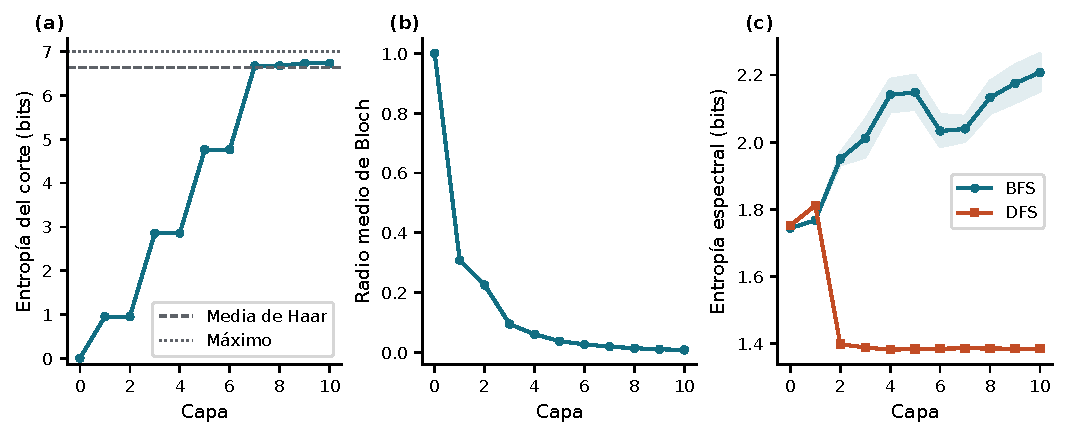
\includegraphics[width=\textwidth]{figures/Fig2_es.pdf}
\caption{Trayectorias de validación: (a) entropía del corte central, distinguiendo media de Haar y máximo; (b) radio medio de Bloch; (c) entropía espectral por modo. El sombreado representa IC puntuales del 95\% por bootstrap de semillas. La igualdad del corte entre profundidades sucesivas sigue el calendario alternado de interacciones}\label{fig:depth}
\end{figure*}

\subsection{Asociaciones estéreo y contrastes entre modos}
RQ3 detecta asociaciones negativas tras BH en profundidades BFS 1, 3 y 4 y DFS 1, 2, 3, 4, 7 y 10. La relación temprana no es uniforme: BFS en profundidad 2 tiene $\rho=-0.198$ y $q=0.096$; DFS presenta relaciones tardías más débiles en 7 y 10 ($\rho=-0.244,-0.262$; $q=0.033,0.021$). En desarrollo hubo asociaciones negativas significativas de 1 a 4 en ambos modos. Se respalda así una relación temprana amplia, pero no la replicación de todo su patrón de significación por capa. La varianza circular describe dispersión azimutal; no es una prueba de preservación de conectividad en estéreo.

La Tabla~\ref{tab:rq4} presenta contrastes pareados. BFS dura aproximadamente 3,30 s menos, tiene menor RMS y mayor ancho de banda y entropía espectral. Su centroide medio es sólo 2,43 Hz mayor, pese a variación mucho mayor entre estados. El flujo pasa de un contraste nulo en desarrollo a una diferencia pequeña en validación ($q=0.0465$). Este resultado secundario se reporta; no demuestra diferencia estadística entre cohortes ni igual relevancia práctica de todos los contrastes.
\begin{table*}[t]
\caption{RQ4: diferencias BFS menos DFS en validación, promediadas por semilla en las 11 capas. IC del 95\% y BH sobre seis contrastes.}\label{tab:rq4}
\centering\small
\begin{tabular}{lrrr}
\toprule
Descriptor & Diferencia media & IC del 95\% & $q$ \\
\midrule
Duración (s) & $-3.301$ & $[-3.348, -3.254]$ & $7.22\times10^{-114}$ \\
RMS digital & $-0.002410$ & $[-0.002460, -0.002359]$ & $1.47\times10^{-97}$ \\
Centroide (Hz) & $2.426$ & $[1.160, 3.710]$ & $3.82\times10^{-4}$ \\
Ancho de banda (Hz) & $51.640$ & $[50.102, 53.187]$ & $3.90\times10^{-82}$ \\
Entropía espectral (bits) & $0.573$ & $[0.560, 0.586]$ & $3.48\times10^{-94}$ \\
Flujo espectral & $0.000789$ & $[0.000050, 0.001568]$ & $0.0465$ \\
\bottomrule
\end{tabular}
\end{table*}


\subsection{Predicción independiente: resultado primario}
El resultado primario de duración DFS satisface el criterio congelado. $M_1$ y $M_2$ tienen MSE de 0,00217588 y 0,00039143 s$^2$. La ganancia es 0,00178445 s$^2$ (IC del 95\% [0,00152409; 0,00206287]), una reducción del 82,01\% del MSE y del RMSE de 46,65 a 19,78 ms (Fig.~\ref{fig:prediction}). El porcentaje describe reducción del error de predicción, no de duración generada ni una mejora perceptual.

La profundidad sola ya predice la duración DFS con precisión: $M_0$ tiene RMSE de 52,31 ms y $R^2=0.998626$. $M_2$ alcanza $R^2=0.999803$; el elevado $R^2$ global debe leerse junto al error absoluto y al modelo base por profundidad. El resultado incremental es una consecuencia replicada de codificación, no el descubrimiento independiente de información cuántica oculta.
\begin{table*}[t]
\caption{RQ5: evaluación independiente con entrenamiento fijo. La reducción de MSE es positiva cuando mejora $M_2$. Sólo duración DFS es objetivo primario. Duración: MSE en s$^2$; flujo: unidades digitales al cuadrado.}\label{tab:rq5}
\centering\small
\begin{tabular}{llrrr}
\toprule
Modo & Objetivo & MSE $M_1$ & MSE $M_2$ & Reducción (\%) \\
\midrule
BFS & Duración & $0.708880$ & $0.709246$ & $-0.05$ \\
BFS & Flujo & $2.04\times10^{-4}$ & $2.04\times10^{-4}$ & $-0.03$ \\
DFS & Duración & $0.002176$ & $3.91\times10^{-4}$ & $82.01$ \\
DFS & Flujo & $1.71\times10^{-6}$ & $1.68\times10^{-6}$ & $1.85$ \\
\bottomrule
\end{tabular}
\end{table*}


Las extensiones BFS para duración y flujo no mejoran MSE y sus IC cruzan cero. El flujo DFS mejora un 1,85\%, con un pequeño IC puntual positivo para ganancia de MSE. Ese intervalo secundario no tiene el estatus confirmatorio del objetivo primario. La asimetría limita cualquier afirmación general de que resúmenes relacionales mejoren todos los objetivos acústicos.

\begin{figure*}[t]
\centering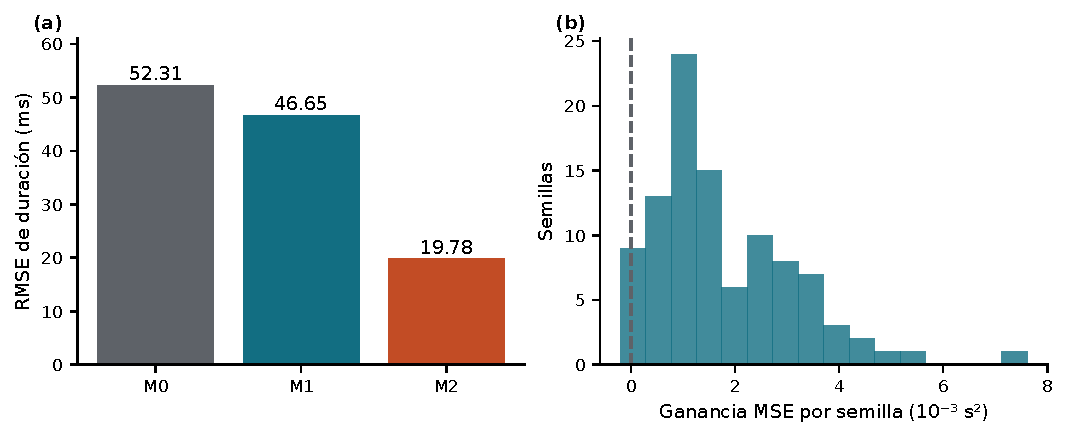
\includegraphics[width=\textwidth]{figures/Fig3_es.pdf}
\caption{Resultado primario de validación. (a) RMSE de duración DFS para modelo por profundidad, modelo local y extensión relacional. (b) Ganancia de error cuadrático por semilla nueva, promediada en 11 profundidades; valores positivos favorecen $M_2$. Modelos y escalado se ajustaron sólo en desarrollo}\label{fig:prediction}
\end{figure*}

\subsection{Explicación mecánica mediante controles}\label{sec:mechanism}
Sean $c$ el número de componentes y $W$ la suma de pesos del bosque en bits. Como un bosque de 15 nodos tiene $15-c$ aristas, su duración ideal DFS es
\begin{align}
T_{\rm DFS}&=0.30c+0.60(15-c)\\
&\quad-0.25W+0.12(c-1)\nonumber\\
&=8.88-0.18c-0.25W\quad\mathrm{s}.\nonumber
\end{align}
Para BFS, sea $F$ el número de fronteras no raíz y $Q$ la suma de sus pesos entrantes medios. Entonces
\begin{equation}
T_{\rm BFS}=0.30c+0.60F-0.25Q+0.12(c-1).
\end{equation}
Estas identidades muestran distintos resúmenes temporales. La duración DFS depende de componentes y peso total del bosque, no de adyacencia etiquetada. BFS depende también de distribución de nodos y pesos entre fronteras. El redondeo por evento define la versión implementada de las ecuaciones.

La reconstrucción independiente de muestras originales DFS coincide con las 1.100 duraciones de validación dentro de $1.78\times10^{-15}$ s. Además, las 16.000 comparaciones de controles DFS tienen diferencia de duración exactamente cero, pese a cambiar adyacencia del árbol en los 400 estados seleccionados. Permutar árbol cambia duración BFS en $-0.4254$ s (IC del 95\% [$-0.5207,-0.3383$]) y número de fronteras en $-0.7905$ ([$-0.9518,-0.6435$]). Permutar pesos conserva fronteras y cambia duración BFS en $+0.01740$ s ([0,01551; 0,01943]), al alterar sus pesos medios. La Fig.~\ref{fig:controls} resume ambas intervenciones.

Los controles respaldan sensibilidad a la organización del bosque y distinguen un invariante de suma de una secuenciación por fronteras. El control de árbol no aísla adyacencia frente a ubicación de pesos o cambios de grado. Duración DFS invariante no implica forma de onda invariante: reordenar y reasignar pesos puede cambiar espectro y estéreo. El suplemento conserva todos los contrastes exploratorios.

\begin{figure*}[t]
\centering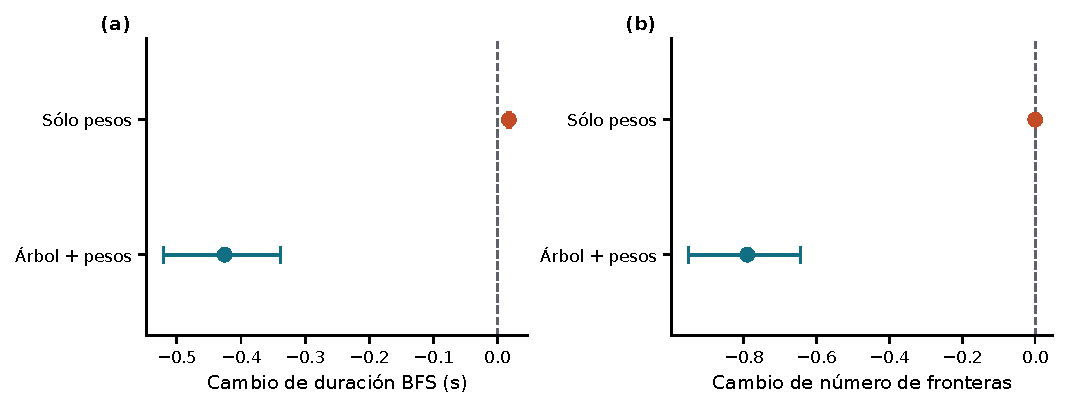
\includegraphics[width=\textwidth]{figures/Fig4_es.pdf}
\caption{Controles sintéticos en validación. Cambios control menos original, promediados entre réplicas y profundidades seleccionadas por semilla. Puntos y barras representan medias e IC puntuales del 95\%. Permutar árbol cambia conectividad y ubicación de pesos; permutar sólo pesos conserva aristas. Ambos mantienen exactamente duración DFS}\label{fig:controls}
\end{figure*}

\subsection{Asociaciones de distancias: replicación parcial}
Se replican asociaciones positivas débiles Bloch--audio: $\rho$ medio por capa de 0,0808 en BFS y 0,1556 en DFS, con BH $q=0.000400$ y BY $q=0.000833$ en ambos (Tabla~\ref{tab:distance}; Fig.~\ref{fig:distance}). La significación no implica concordancia geométrica fuerte ni similitud perceptual. No se especificó una prueba directa de diferencia entre correlaciones de modos.

La familia de validación no respalda distancias de información mutua--audio: BFS $\rho=-0.0103$, $q=0.539$; DFS $\rho=0.0330$, $q=0.097$. El valor exploratorio DFS en desarrollo fue $\rho=0.0536$, $q=0.00213$. La no replicación es compatible con la fuerte predicción de duración DFS: resúmenes útiles de pesos no tienen por qué conservar distancias de matrices completas. Un resultado no significativo tampoco demuestra independencia exacta ni asociación poblacional nula.
\begin{table*}[t]
\caption{Distancias en validación: media no ponderada de Spearman por capa, 5.000 permutaciones de semillas completas y correcciones en cuatro pruebas. Bloch: capas 1--10; MI: 2--10.}\label{tab:distance}
\centering\small
\begin{tabular}{llrrrr}
\toprule
Modo & Descriptor & $\bar\rho$ & $p$ & $q_{\rm BH}$ & $q_{\rm BY}$ \\
\midrule
BFS & Bloch & $0.0808$ & $0.000200$ & $0.000400$ & $0.000833$ \\
BFS & MI & $-0.0103$ & $0.539092$ & $0.539092$ & $1.000000$ \\
DFS & Bloch & $0.1556$ & $0.000200$ & $0.000400$ & $0.000833$ \\
DFS & MI & $0.0330$ & $0.072785$ & $0.097047$ & $0.202182$ \\
\bottomrule
\end{tabular}
\end{table*}

\begin{figure*}[t]
\centering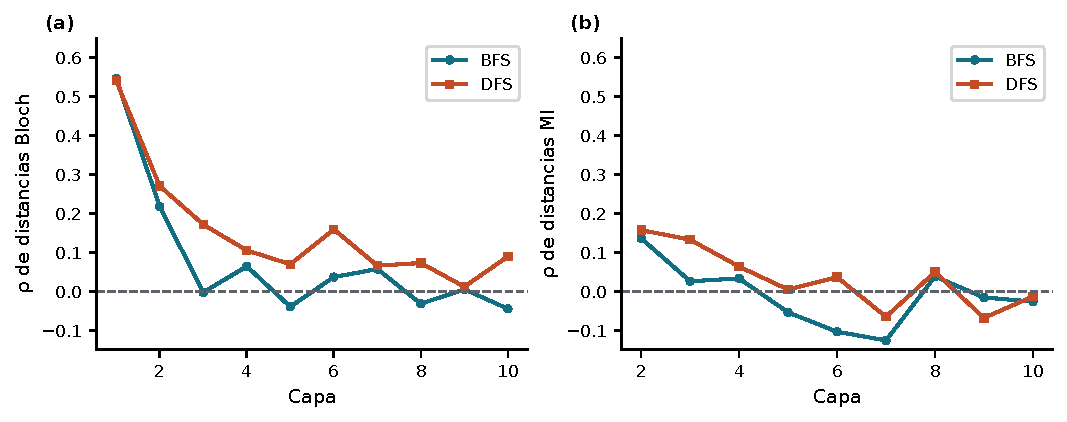
\includegraphics[width=\textwidth]{figures/Fig5_es.pdf}
\caption{Correlaciones de distancias dentro de cada profundidad de validación para (a) descriptores cartesianos de Bloch alineados y (b) matrices completas de información mutua. La prueba global promedia las correlaciones mostradas y permuta etiquetas completas de semilla entre profundidades. La regla numérica fija excluye capas degeneradas. Las curvas no presentan bandas inferenciales}\label{fig:distance}
\end{figure*}

\subsection{Límite constructivo a la inferencia global}\label{sec:nogo}
Una representación basada en reducciones seleccionadas puede ocultar entrelazamiento global realmente distinto. La relación general entre marginales de estados de grafo y estructura multipartita está establecida en información cuántica \citep{Hein2004,Vandre2025}; la siguiente construcción explicita el límite para este motor.

\textbf{Proposición.} Se prepara $|+\rangle^{\otimes15}$, se aplican compuertas controladas-$Z$ en un ciclo de siete nodos dentro de $A$ y otro de ocho dentro de $B$, y $\operatorname{CP}(\alpha_i)=\operatorname{diag}(1,1,1,e^{\mathrm i\alpha_i})$ en los siete pares $(i,7+i)$, $i=0,\ldots,6$. Para fases reales arbitrarias, todas las reducciones de uno y dos qubits son máximamente mixtas, pero
\begin{equation}
S_A=\sum_{i=0}^{6}h_2\left(\sin^2\frac{\alpha_i}{4}\right),
\end{equation}
donde $h_2$ es entropía binaria. Con descriptores exactos, $\alpha_i=\pi t$, $0\le t\le1$, define una familia continua con $S_A\in[0,7]$ bits y audio de instantánea final idéntico dentro de cada modo y configuración fijos.

La prueba cancela toda coherencia de uno o dos qubits mediante un vecino del ciclo interno que se traza y no recibe contribución del emparejamiento entre bloques. Las compuertas internas son locales respecto de $A|B$ y conmutan con el emparejamiento; el espectro del corte corresponde así a siete pares independientes de fase controlada. El Recurso en línea 1 contiene prueba completa y certificado exhaustivo de 330 casos. Diecisiete estados numéricos, con fases también heterogéneas, corroboran marginales y fórmula de entropía. Las verificaciones archivadas con el motor congelado dan muestras idénticas por modo. Son preparaciones físicas externas, no circuitos del conjunto RQC ni controles sintéticos de información mutua. Para $S_A=0$, cada bloque sigue entrelazado internamente.

Como la onda final es constante en esta familia, cualquier estimador que recibe sólo esa onda tiene error absoluto esperado de peor caso óptimo de al menos 3,5 bits y error cuadrático medio de al menos 12,25 bit$^2$ para entropía del corte; el estimador constante del punto medio alcanza ambas cotas. Se excluye recuperación universal incluso por estimadores aprendidos o aleatorizados, sin excluir predicción en una distribución restringida ni inferencia con observables adicionales, metadatos identificadores o historial de preparación. La construcción caracteriza esta representación sin reclamar prioridad para el fenómeno general de marginales.

\subsection{Discontinuidad de coordenadas del paneo congelado}
El mapeo de azimut módulo $2\pi$ tiene una discontinuidad en $\phi=0\equiv2\pi$. Dos estados puros ecuatoriales con azimut $\pm\epsilon$ tienen distancia de traza $\sin\epsilon\to0$, pero sus ganancias se aproximan a canales opuestos. Para una misma voz aislada se normaliza la diferencia estéreo por la raíz de la suma de energías de ambas señales. Su cuadrado es $1-\sin(\epsilon/2)\to1$ (Fig.~\ref{fig:limits}). El determinismo no implica continuidad global respecto de distancia física entre estados. Neutralizar dirección a radio cero no elimina la discontinuidad con radio no nulo. Conservamos la regla congelada y documentamos su límite; sustituirla por una continua definiría nueva versión del instrumento y dataset.

\begin{figure*}[t]
\centering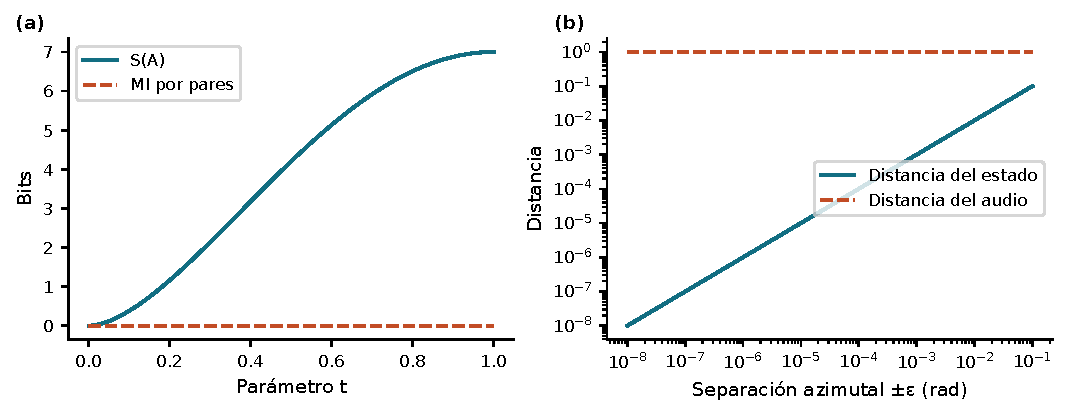
\includegraphics[width=\textwidth]{figures/Fig6_es.pdf}
\caption{Límites analíticos, separados de validación RQC. (a) La familia física de fase controlada tiene entropía del corte variable e información mutua por pares nula y produce audio final idéntico por modo. (b) Al cruzar la discontinuidad azimutal, la distancia de traza del estado tiende a cero y la distancia normalizada del audio de una voz tiende a uno. Ambas curvas siguen fórmulas exactas}\label{fig:limits}
\end{figure*}

\section{Discusión}\label{sec:discussion}
\subsection{Qué codifica el instrumento}
Los resultados respaldan una representación selectiva. Los descriptores de Bloch presentan asociaciones acústicas agregadas replicadas y los resúmenes relacionales reducen sustancialmente un error concreto en circuitos nuevos. Las identidades temporales y controles explican por qué: DFS comprime peso del bosque en duración total, mientras BFS responde también a organización de fronteras. Son restricciones útiles para diseñar y explicar el instrumento. No implican correspondencia exclusiva entre cada característica audible y una cantidad cuántica ni recuperación del estado desde la señal final.

Es esencial distinguir grafo completo y bosque. $M_2$ utiliza resúmenes del grafo completo; DFS secuencia directamente pesos del bosque. La predicción validada es una relación del conjunto de circuitos entre esos resúmenes y la regla temporal, no una demostración de conservar geometría matricial completa. La no replicación de distancias de información mutua muestra empíricamente ese límite. Recuperar topología desde duración DFS contradice su invariante exacto; recuperar entrelazamiento central arbitrario desde audio contradice el certificado físico.

Las mesetas de entropía se interpretan sin introducir física especulativa. Siguen invariancia ante unitarias locales respecto de un corte y el calendario alternado de interacciones que lo cruzan. La entropía es no negativa, su máximo es dimensional y Page proporciona una media de Haar. Grafos, entropía y semejanza con una escalera no aportan aquí evidencia de espacio-tiempo emergente, holografía ni geometría de amplituedros. Tales analogías quedan fuera del aporte demostrado.

\subsection{Implicaciones multimodales y compositivas}
La tarea audiovisual más defendible es inspeccionar correspondencias: seleccionar semilla y capa, ver vectores de Bloch y grafo completo junto a su bosque, y comparar BFS y DFS. Una interfaz sincronizada podría resaltar nodos/fronteras activos y mostrar la regla temporal exacta. Es una implicación de diseño del motor verificado, no evaluación de una interfaz implementada en este estudio. Antes de sostener afirmaciones de interfaz, deben documentarse por separado sus controles reales, sincronización, capturas y flujo de tarea.

El certificado físico ofrece un ejemplo pedagógico útil: las mismas representaciones local y por pares y el mismo sonido pueden acompañar distinto entrelazamiento en una partición mayor. Distingue resumen de subsistemas y propiedad global. Los controles, a su vez, muestran cómo voces fijas adquieren distintas formas temporales mediante organización relacional. Pueden sustentar explicaciones o ejercicios compositivos; mejorar aprendizaje o escucha sigue siendo una pregunta empírica.

Respecto de métodos que sonifican directamente entropía bipartita \citep{Tudoce2026}, aquí la entropía del corte es un observable de análisis y no un parámetro tímbrico directo. Respecto de Q1Synth \citep{Miranda2023}, el énfasis está en secuenciación relacional multiqubit y evaluación entre circuitos. Son decisiones complementarias. No se realizó un benchmark perceptual o computacional compartido ni se establece superioridad.

\subsection{Limitaciones y alcance}
La generalización se restringe a circuitos ideales de 15 qubits, profundidades 0--10 y raíz, etiquetas, tolerancia y síntesis fijas. Las semillas son identificadores seudoaleatorios reproducibles de trayectorias, no muestras de todos los estados cuánticos. La cohorte prospectiva aborda selección entre estos circuitos; no prueba robustez ante ruido, hardware, otras compuertas, números de qubits, raíces ni escalado asintótico. La simulación exacta sigue siendo exponencialmente costosa aunque sólo se produzcan 15 voces. La familia analítica prueba falta universal de inyectividad entre estados físicos; las conclusiones estadísticas siguen dependiendo de la distribución estudiada.

BFS y DFS cambian simultáneamente varias decisiones, por lo que RQ4 no atribuye diferencias sólo al orden del recorrido. El bosque selecciona aristas con pérdida de información; permutar árbol modifica varias propiedades; las distancias acústicas incluyen duración. Asociaciones débiles de distancias, IC puntuales de controles y asociaciones secundarias modestas o inestables no deben presentarse como preservación completa. La discontinuidad de paneo limita continuidad y puede amplificar cambios azimutales próximos a su frontera. Los descriptores digitales no sustituyen pruebas auditivas y no se realizó estudio con oyentes, usuarios ni de aprendizaje.

\section{Conclusiones}
El motor congelado de Bloch e información mutua se caracteriza como representación selectiva con consecuencias acústicas reproducibles. La validación independiente respalda asociaciones locales y una fuerte mejora incremental de predicción de duración DFS; los controles muestran que esa duración codifica suma de pesos del bosque, no conectividad completa. Las asociaciones de distancias de Bloch se replican débilmente y la preservación de distancias de información mutua no recibe respaldo de validación. Una familia física continua demuestra que la entropía central puede recorrer todo su intervalo mientras el audio final permanece constante. Estos resultados establecen qué mide, organiza y no puede identificar el instrumento. Proporcionan una base computacional para exploración audiovisual documentada y composición, dejando beneficios humanos para evaluación específica.

\backmatter
\section*{Información suplementaria}
El Recurso en línea 1 contiene tablas ampliadas, todos los contrastes secundarios de controles y pruebas de identidades temporales, certificado físico y discontinuidad azimutal. El Recurso en línea 2 contiene datos de análisis, especificaciones congeladas, hashes, certificados numéricos y scripts de reproducción. Ambas versiones lingüísticas presentan la misma evidencia; el español se proporciona para revisión del equipo.

\section*{Declaraciones}
\textbf{Disponibilidad de datos y código.} El repositorio es \url{https://github.com/valirus/Quantum-Sonification-Bloch-V1}. El paquete reproducible complementario contiene tablas de desarrollo y validación, predicciones registradas, resultados compactos completos, protocolo congelado y código del sintetizador de referencia. El archivo completo de evidencia incluye matrices y metadatos por semilla; los vectores de estado, circuitos y WAV completos se conservan en las ejecuciones del proyecto. Antes del envío, los autores deben completar un identificador de depósito permanente versionado y disponibilidad pública de los commits de análisis citados; no se presenta la URL del repositorio como depósito de esos archivos.

\textbf{Participantes humanos.} Los experimentos reportados utilizan simulación clásica y análisis de señales, sin participantes ni datos personales de participantes.

\textbf{Asistencia de IA.} ChatGPT/Codex asistió redacción, traducción, preparación de scripts y verificaciones de consistencia. Las conclusiones se fundamentan en registros suministrados, datos inspeccionables y cálculos reproducibles. Esta asistencia no establece autoría; los autores humanos deben verificar y aprobar texto, análisis y referencias finales.

\textbf{Financiación, conflictos de interés y contribuciones.} El equipo debe completar y aprobar estas declaraciones específicas, nombres, afiliaciones y datos de correspondencia antes del envío. No se infiere ausencia de financiación ni de conflictos.

\bibliography{references}
\end{document}
